\documentclass[11pt]{article}
\usepackage{coling2014}
\usepackage{times}
\usepackage{url}
\usepackage{latexsym}



\usepackage{fontspec}
\usepackage{xunicode}
\usepackage{xltxtra}

\usepackage{graphicx}
\usepackage{caption}
\usepackage{subcaption}

\title{Hyper-minimization of Finite state Lexicions Using Flag Diacritics}


\author{First Author \\
  Affiliation / Address line 1 \\
  Affiliation / Address line 2 \\
  Affiliation / Address line 3 \\
  {\tt email@domain} \\\And
  Second Author \\
  Affiliation / Address line 1 \\
  Affiliation / Address line 2 \\
  Affiliation / Address line 3 \\
  {\tt email@domain} \\}

\date{}

\begin{document}
\maketitle
\begin{abstract}
  max 200 words
\end{abstract}




\section{Introduction}
%
% The following footnote without marker is needed for the camera-ready
% version of the paper.
% Comment out the instructions (first text) and uncomment the 8 lines
% under "final paper" for your variant of English.
% 
\blfootnote{
    %
    % for review submission
    %
    %\hspace{-0.65cm}  % space normally used by the marker
    %Place licence statement here for the camera-ready version, see
    %Section~\ref{licence} of the instructions for preparing a
    %manuscript.
    %
    % % final paper: en-uk version (to license, a licence)
    %
    % \hspace{-0.65cm}  % space normally used by the marker
    % This work is licensed under a Creative Commons 
    % Attribution 4.0 International Licence.
    % Page numbers and proceedings footer are added by
    % the organisers.
    % Licence details:
    % \url{http://creativecommons.org/licenses/by/4.0/}
    % 
    % % final paper: en-us version (to licence, a license)
    %
     \hspace{-0.65cm}  % space normally used by the marker
     This work is licenced under a Creative Commons 
     Attribution 4.0 International License.
     Page numbers and proceedings footer are added by
     the organizers.
     License details:
     \url{http://creativecommons.org/licenses/by/4.0/}
}

\section{Background}
\label{sec:background}

 
\section{Flag diacritics}
\label{sec:flags}

Flag diacritics are special multi-character symbols which are interpreted during runtime. They can be used to optimize large transducers to couple entrance points of the sub-graphs with the correct exit points.

Their special syntax is: \verb+@operator.feature.value@+, where
\texttt{operator} is one of the available operators (P, U, R, D, N, C), \texttt{feature} is the name of a feature set by the user and \texttt{value} can be any value held in a feature, also provisionally defined. For additional information on the semantics of flag diacritic operators, see~\newcite{beesley2003finite}.


In this paper, we will use only two types of flag diacritics: positive
setting (\verb+@P.feature.value@+) and require test
(\verb+@R.feature.value@+). While positive setting flag only sets the
feature to its value, the require test flag invokes testing whether the
feature is set to the designated value. For example,
\verb+@P.LEXNAME.Root@+ will set feature \texttt{LEXNAME} to value
\texttt{Root}. If later in the path there is an R flag that requires test
\verb+@R.LEXNAME.Root@+, the invoked test will succeed and that path
will be considered valid.


\section{Notation}
\label{sec:notation}
TODO ...


\begin{table}[h]
    \centering
    \begin{tabular}{|c|c|}
        \hline
        \bf Operation & \bf Name \\
        \hline\hline
        \bf a b & concatenation  \\
        \bf a | b & disjunction  \\
        \bf a : b & cross product  \\
        \bf a .o. b & composition  \\
        \bf * & Kleene star  \\
        

        \hline
    \end{tabular}
    \caption{List of operators
    \label{table:operators}}
\end{table}




\section{Methods}
\label{sec:methods}


\begin{figure}[htbp]
    \centering

\begin{subfigure}[t]{0.3\textwidth}
\begin{verbatim}
LEXICON Root
A ;
B ;
C ;

LEXICON A
aaa A ;
# ;

LEXICON B
aaaa B ;
# ;

LEXICON C
aaaaa C;
#;
\end{verbatim}
\caption{Lexc grammar description
\label{fig:lexc-a2}}
\end{subfigure}
 ~ %add desired spacing between images, e. g. ~, \quad, \qquad etc.
\begin{subfigure}[t]{0.3\textwidth}
\begin{verbatim}
ORIGINAL:
no. of states: 60
no. of arcs: 60
no. of final states: 36
\end{verbatim}
\caption{Summary of the transducer without flag diacritics
\label{fig:sizes-orig}}
\end{subfigure}%
 ~ %add desired spacing between images, e. g. ~, \quad, \qquad etc.
\begin{subfigure}[t]{0.3\textwidth}
\begin{verbatim}
HYPER-MINIMAL:
no. of states: 23
no. of arcs: 27
no. of final states: 1
\end{verbatim}
\caption{Summary of the hyper-minimal transducer
\label{fig:sizes-flags}}
 \end{subfigure}

 \caption{Simple example lexicon with transducer sizes}
 \label{fig:simple-ex}
\end{figure}


This algorithm is an improvement of hyper-minimization algorithm introduced in~\newcite{drobac2014}. The main idea of the algorithm is to 
replicate structure of a morphological lexicon into a finite state transducer with use of flag diacritics. Every sub-lexicon should start 
with require flag \verb+R.LEXNAME.sub-lex+, where \verb+LEXNAME+ is feature name that we use for this special purpose
and \verb+sub-lex+ is name of the current sub-lexicon. Accordingly, every continuation should be expressed with positive setting flag 
\verb+P.LEXNAME.sub-lex+, which sets feature \verb+LEXNAME+ to a \verb+sub-lex+ value, which corresponds to the continuation lexicon.
TODO - example?

\begin{figure}
\centering
\begin{subfigure}[b]{0.4\textwidth}
        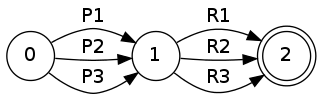
\includegraphics[width=\textwidth]{hub.png}
        \caption{A hub state}
        \label{fig:hub}
\end{subfigure}%
\quad %add desired spacing between images, e. g. ~, \quad, \qquad etc.
  %(or a blank line to force the subfigure onto a new line)
\begin{subfigure}[b]{0.4\textwidth}
        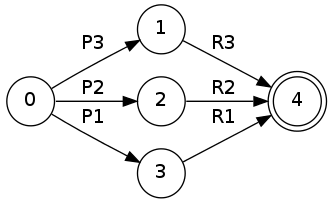
\includegraphics[width=\textwidth]{distr.png}
        \caption{Distributed hub}
        \label{fig:distr}
\end{subfigure}
\caption{Hub state before and after distribution}
\label{fig:hub_distr}
\end{figure}


While in the previous version flags were concentrated in flag diacritic hubs, single states from where all continuation lexicons begin with a 
require test 
and end with positive settings, new method distributes flag diacritic states. For example, if one hub state would have incoming transitions 
$P_1$, $P_2$, $P_3$ and outgoing transitions $R_1$, $R_2$, $R_3$, the distributed version would be divided into three states, each with one 
$P_i$ $R_i$ pair, as shown in 
Figure~\ref{fig:hub_distr}. Therefore, we can say:

\begin{equation}\label{hub_replacement}
[P_1 | P_2 | P_3] [R_1 | R_2 | R_3] \rightarrow [P_1 R_1] | [P_2 R_2] | [P_3 R_3]
\end{equation}



This distributiveness is necessary because it allows 
composition of lexicon with grammar rules without creating extra invalid flag diacritic paths, which means that, 
unlike in the previous version, there is no need for pruning after the composition.


One of the examples why preserving the lexical structure with flag diacritics is useful is explained on a small scale artificial example shown in 
Figure~\ref{fig:simple-ex}.
 
The Figure~\ref{fig:lexc-a2} shows language description of the following language: $(aaa)^*|(aaaa)^*|(aaaaa)^*$, written in 
the \texttt{lexc} format. In case this language is compiled into a normal, minimal transducer, it will consist of 60 states and 60 arcs, 
but with the hyper-minimal method, the transducer size will be less then half of it: 23 states and 27 arcs, as shown in 
Figure~\ref{fig:sizes-orig} and Figure~\ref{fig:sizes-flags} respectively.

This happens because the non-flagged transducer will try to combine and keep all possible options of strings in the same path, until it gets 
the least common multiple of strings $aaa$, $aaaa$ and $aaaaa$. On the other hand, the flagged version will be able to distribute those three 
strings to different paths, avoiding duplication as much as possible.

If we define transducer depths as the length of the longest path from any state to another state that doesn't go through the same state twice, 
the non-flagged version has maximal depth of 59 after which it returns to the starting state to complete the cycle, while the hyper-minimal 
one has maximal depth of 9. Keeping the transducer shallow will reduce the necessary number of states and paths, which results in smaller final size.

The similar combinatorial phenomena occur in large lexicons, like in Greenlandic, but it is difficult to find illuminating and small real 
world examples that could be presented in a paper.


\begin{figure*}
    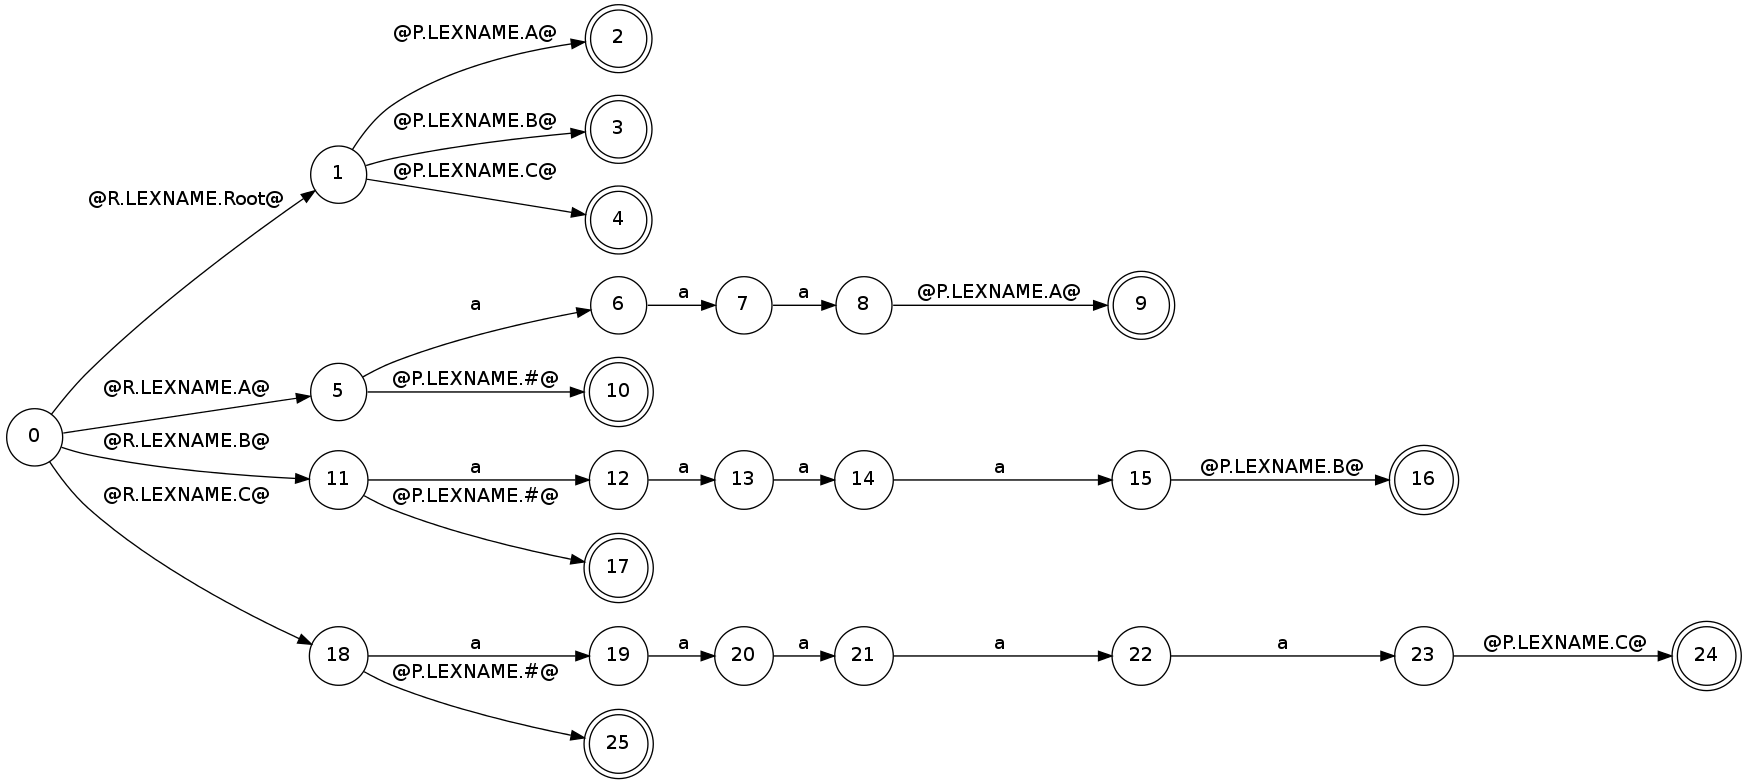
\includegraphics[width=\textwidth]{trie.png}
     \caption{First step is to build a lexical trie
     \label{fig:trie}}
\end{figure*}


\begin{figure*}
    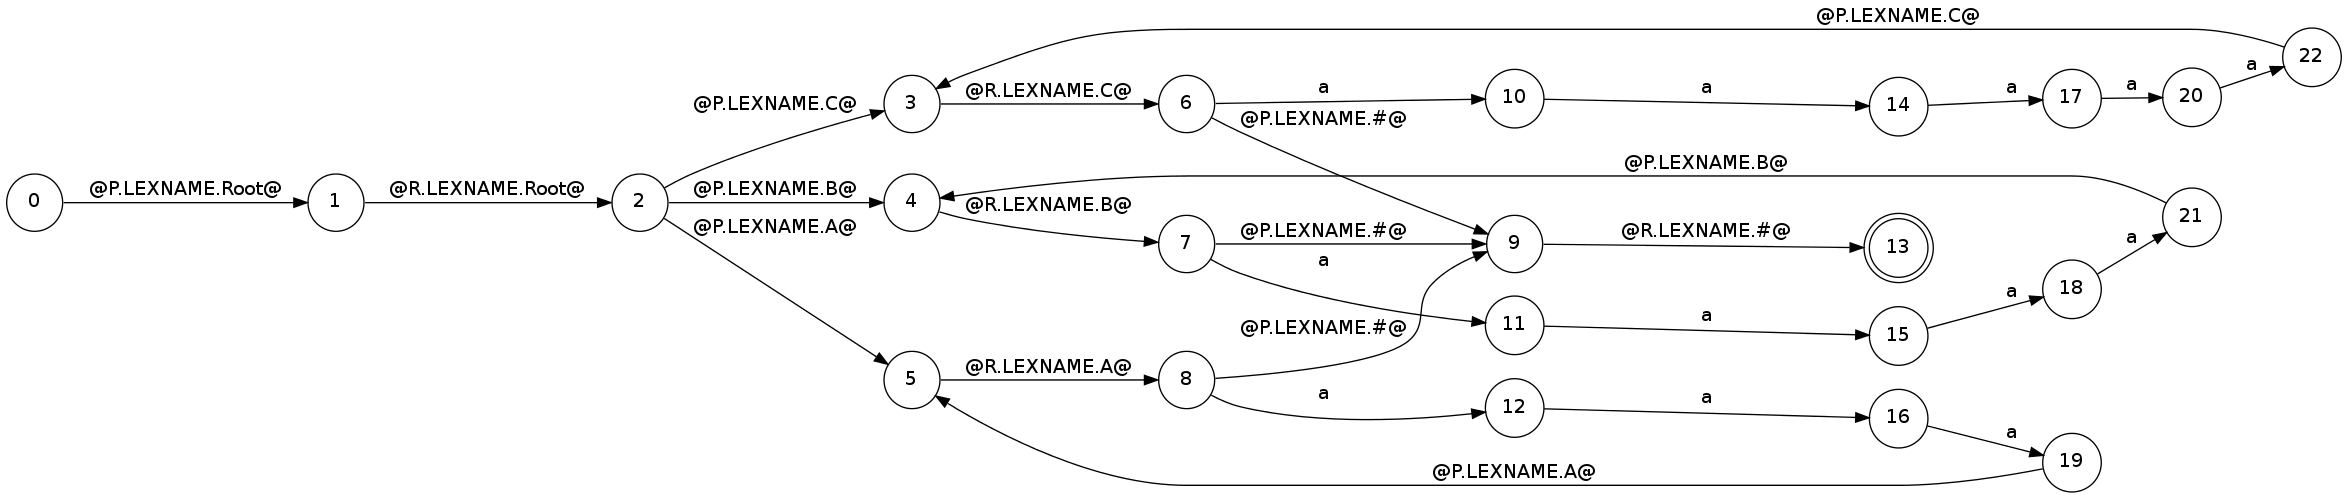
\includegraphics[width=\textwidth]{after_comp.png}
     \caption{Transducer after composition with filter
     \label{fig:after}}
\end{figure*}



\subsection{Lexical compilation}

Previous version of \texttt{lexc} took to long to compile because each sub-lexicon was build separately and then disjunct with others. Compilation time of large morphologies would take up to several hours. In order to improve compilation speed and incorporate hyper-minimization part, we needed to change the \texttt{lexc} algorithm.

First, from a lexical description we build a transducer trie, an ordered, acyclic finite state transducer. In the trie, every sub-lexicon 
starts from the same start state with a require flag with a sub-lexicon name as a value. After the require flag, continues the morph, followed 
by a positive setting flag with continuation value. In a case where the morph is a pair of two strings, epsilon padding is added to the end of 
the shorter string.

\texttt{Lexc} can also contain regular expressions. In that case, the regular expression is parsed and processed into a transducer which is saved into 
a map of regular expression keys and matching transducers. The key is added to the trie the same way the strings are - trie entry will start with 
the encoded sub-lexicon name, followed by regular expression key and finish with the continuation. Later in the process, the regular expression 
keys are substituted with matching transducers from the map. 
Example of a trie built from lexical description in Figure~\ref{fig:lexc-a2} is shown in Figure~\ref{fig:trie}.

When the entire lexical file is read into a trie, the trie is transformed into a transducer and over-generated with Kleene star:
\begin{equation}\label{eq:trie_star}
tr = \left[f(trie)\right]^* 
\end{equation}
Transformation of the trie to a transducer is fast operation, even for large data structures, which results in fast and efficient \texttt{lexc}.

The next step is concatenation of starting and ending encoded joiners to the beginning and the end of the transducer. 
%(In case of non-flagged version, the starting joiner is initial lexicon name, usually \texttt{Root} and ending joiner is encoded final lexicon, \texttt{\#}.)
In case of the hyper-minimized transducer, the starting joiner is encoded P flag of the initial sub-lexicon, usually \texttt{P.LEXNAME.Root} and the ending one is R flag of the final lexicon, \texttt{R.LEXNAME.\#}.

\begin{equation}\label{eq:joiners}
tr' = \verb+P.LEXNAME.Root + tr \verb+ R.LEXNAME.#+
\end{equation}
This way, the transducer will always start and end with the same flag pair.

To filter out invalid flag diacritic paths, caused by trie over-generation from equation~\ref{eq:trie_star}, the transducer is composed to filter:
\begin{equation}\label{eq:composition}
tr'' = tr' .o. filter
\end{equation}
where filter is:
\begin{equation}\label{eq:filter}
filter = \left[ \left(\bigcup_{i} \verb+P.LEXNAME+_i \verb+ R.LEXNAME+_i \right) \cup (\Sigma \setminus F) ^*\right]^* 
\end{equation}

In a case some flag pairs are wished to be left out from the transducer, at this point the flag pairs could be replaced with epsilon.


The final step is to replace regular expression keys with actual regular expression transducers
\begin{equation}\label{eq:regex}
regular\_expession\_key \rightarrow regular\_expression\_transducer
\end{equation}

In Figure~\ref{fig:after} is shown the final hyper-minimal transducer built from lexical description from Figure~\ref{fig:lexc-a2}. 




\section{Results}
In Table~\ref{table:sizes} we show sizes of the morphological analyzer built with different approaches. The first column shows analyzer 
size without any flag diacritics, it is followed by sizes achieved with the previous method and finally there are shown sizes when 
compiled with the method proposed in this paper.
\begin{table}
    \centering
    \begin{tabular}{|l|r|r|r|r|r|}
        \hline
        \bf Language & \bf Original & \bf Old flags  & \bf \% & \bf New flags  & \bf \% \\
        \hline\hline
        \bf Greenlandic &   168 M  & 17 M & 10,1\% &  14 M & 8,3\% \\
        \bf North Saami &   12 M    & 5,7 M & 47,5\% & 10 M & 83,3\% \\
        \bf Finnish &   17 M    & 16 M & 94,1\% & 16 M & 94,1\% \\
        \bf Lule Saami  &   5 M    & 3 M & 60,0\% & 5 M & 100\% \\
        \bf Erzya       &   3,7 M    & 5,3 M & 143,2\% &  5 M & 135,13\% \\
        \hline
    \end{tabular}
    \caption{Analyzer size - Sizes of transducers without and with automatic flags (in megabytes); Percentage shows size of the flagged transducer in comparison with the original
    \label{table:sizes}}
\end{table}

In Table~\ref{table:lookup} we show lookup speed of the morphological analysers expressed in words per second...

\begin{table}[h]
 \centering
    \begin{tabular}{|l|r|r|r|r|r|}
        \hline
        \bf Language & \bf Original & \bf Old version & \bf \% & \bf New version & \bf \% \\
        \hline\hline
        \bf Greenlandic & 2 770 w/s & 2 507 w/s & 90,5\% & 2072 w/s & 74,8\%  \\
        \bf North Saami & 30 714 w/s & 8 775 w/s & 28,6\% & 11 168 w/s & 36,4\%  \\
        \bf Finnish  & 84 415 w/s & 27 420 w/s & 32,5\%  & 28 615 w/s & 33,9\%  \\
        \hline
    \end{tabular}
    \caption{Look-up speed of transducers without and with automatic flags; Percentage shows speed of the flagged transducer in comparison with the original
    \label{table:lookup}}
\end{table}


% Find out and discuss why tr with lots of flags get big after applying rules

\section{Data}
\label{sec:data}

We measure the success of our algorithm using real-world, large-scale
language descriptions. For this purpose we have acquired freely
available, open source language descriptions from the language repository of the University of 
Tromsa~\cite{moshagen2013building}.\footnote{https://victorio.uit.no/langtech, revision 90691} The
languages selected are Greenlandic (kal), North Saami (sme), Erzya
(myv), Finnish (fin) and Lule Sami (smj).

All operations with transducers were performed using Helsinki Finite
State Technology tools~\cite{linden2011}.\footnote{svn.code.sf.net/p/hfst/code, revision 3813}



\section{Discussion}
\label{sec:discussion}



%\subsection{Future Directions}
%\label{subsec:future-directions}

%This is an optimistic thing so we thought that automatic induction of flags
%shoulda work nicely for other neat things too. Hyper-minimization based on
%morphophonology would be cool. Also, graph-structure. And other things.

\section{Conclusion}
\label{sec:conclusion}



\iffalse
\section*{Acknowledgements}
The research leading to these results has received funding from FIN-CLARIN, Langnet and the
European Commission's 7th Framework Program under grant agreement n° 238405 (CLARA).
\fi

\bibliographystyle{acl}
\bibliography{hyperminimization-with-lexc2.bib}




\end{document}


